\documentclass[a4paper,11pt,dvipdfmx]{jsarticle}


% 数式
\usepackage{amsmath,amsfonts}
\usepackage{bm}

% 画像
\usepackage[dvipdfmx]{graphicx}

% 図形
\usepackage{tikz}
\usetikzlibrary{shapes.geometric}
\usetikzlibrary {shapes.misc}
\usepackage{tikz-imagelabels}

% ソースコード
\usepackage{listings,jlisting,color}
\lstset{
basicstyle={\ttfamily},
identifierstyle={\small},
commentstyle={\smallitshape},
keywordstyle={\small\bfseries},
ndkeywordstyle={\small},
stringstyle={\small\ttfamily},
frame={tb},
breaklines=true,
columns=[l]{fullflexible},
numbers=left,
xrightmargin=0zw,
xleftmargin=3zw,
numberstyle={\scriptsize},
stepnumber=1,
numbersep=1zw,
lineskip=-0.5ex
}
\renewcommand{\lstlistingname}{ソースコード}


\begin{document}

\title{画像処理 課題1 トーンマッピング}
\author{21T2166D 渡辺大樹}
\date{2023/05/25}
\maketitle

\section{課題の目的・意図}
本課題では、ヒストグラムの幅(画像の輝度値の範囲)を広げる線形濃度変換と
逆光時などの明るさにばらつきが出た画像のヒストグラムの局所的、急激な変化の山を改善するヒストグラム平坦化を
用いて、コントラストの強調された、また明るさのばらつきが少ない画像を得ることを目的とし行う。

\section{処理内容}
以下では線形濃度変換とヒストグラム平坦化の二つの処理で実際に行っていることを説明していく。
\subsection{線形濃度変換}
線形濃度変換では低コントラスト、言い換えれば露出度が適切ではない画像の輝度値を解析し、その分布範囲を線形関数
を用いて広くすることで、色差の大きい画像を生成する。すなわち図\ref{hist_1}のような変換を行う。
\begin{figure}[htbp]
    \centering
    \begin{minipage}{0.4\hsize}
        \centering
        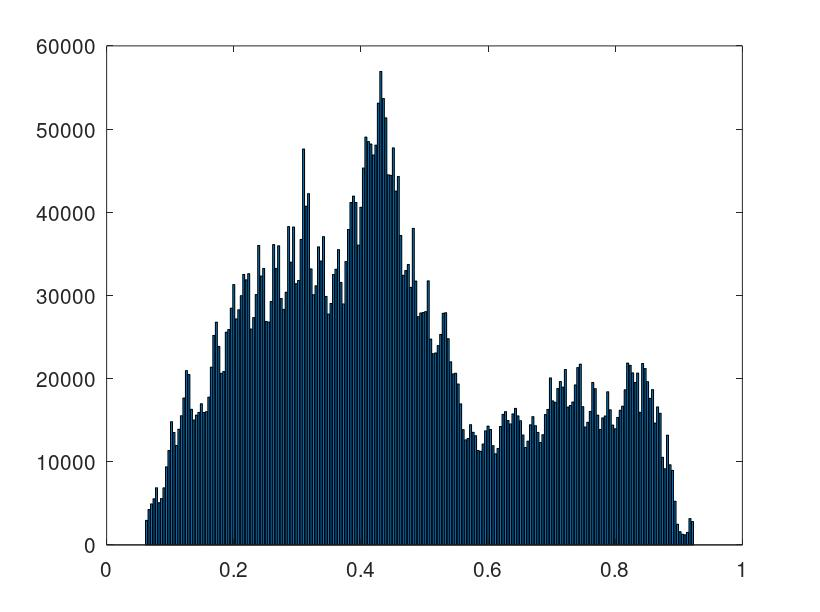
\includegraphics[width=50mm]{./img/linear_ex.jpg}
    \end{minipage}
    \begin{minipage}{0.1\hsize}
        \centering
        \begin{math}
                \overset{f(x)=ax+b}{\to}
        \end{math}
    \end{minipage}
    \begin{minipage}{0.4\hsize}
        \centering
        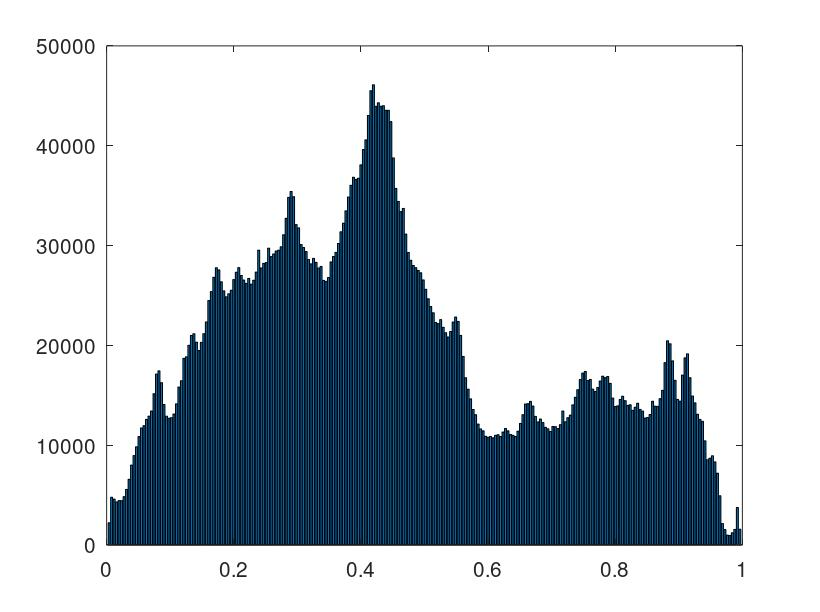
\includegraphics[width=50mm]{./img/linear_ex1.jpg}
    \end{minipage}
    \caption{線形濃度変換によるヒストグラムの変化例}
    \label{hist_1}
\end{figure}

そのためには処理前の画像から得られた輝度値から、その輝度値の範囲を確認。この変換前の輝度値の範囲を$x_1,x_2(x_1<x_2)$とすると、
これを輝度値の最大、最小値まで拡大するような線形関数を、この画像の輝度値全体に適応する必要がある。

入力画像の輝度値の範囲を$x_1,x_2$とし、出力画像の輝度値の範囲を$y_1,y_2$とする。

$y=ax+b$の形の線形関数を用いて変形を行うとき(この変形はアフィン変換という)定数である$a,b$は連立方程式

\begin{equation}
    \left \{ \,
    \begin{aligned}
        y_1 &= ax_1 + b \\
        y_2 &= ax_2 + b
    \end{aligned}
    \right .
\end{equation}
を解くことで求まる。これは$a,b$の係数行列と$(a,b)$の積であると考えれば

\begin{equation}
    \begin{pmatrix}
        y_1 \\ y_2
    \end{pmatrix}
    =
    \begin{pmatrix}
        x_1 & 1 \\
        x_2 & 1
    \end{pmatrix}
    \begin{pmatrix}
        a \\ b
    \end{pmatrix}
\end{equation}
となる。これは逆行列を用いて解くことができて、

\begin{equation}
    \frac{1}{x_1-x_2}
    \begin{pmatrix}
        y_1 - y_2 \\ -x_2y_1 + x_1y_2
    \end{pmatrix}
    =
    \begin{pmatrix}
        a \\ b
    \end{pmatrix}
\end{equation}
としてしまえば、

\begin{equation}
    \left \{ \,
    \begin{aligned}
        a &= \frac{y_1-y_2}{x_1-x_2} \\
        b &= \frac{-x_2y_1+x_1y_2}{x_1-x_2}
    \end{aligned}
    \right .
\end{equation}
と求まる。

これにより求まった式(4)の係数を利用するのが線形濃度変換の計算方法となる。

このヒストグラムの濃度変換はほかにも、
いくつかの区分の一次式、多項式を組み合わせたもの(スプライン関数)や$\tan$関数などを用いることもある。

\subsection{ヒストグラム平坦化}
続いて、逆光時など明るさにばらつきがある画像を補正する処理、ヒストグラム平坦化について説明していく。

逆光などで明るさのばらつく画像は図\ref{hist_2}のようなヒストグラムになっている。
\begin{figure}[htbp]
    \centering
    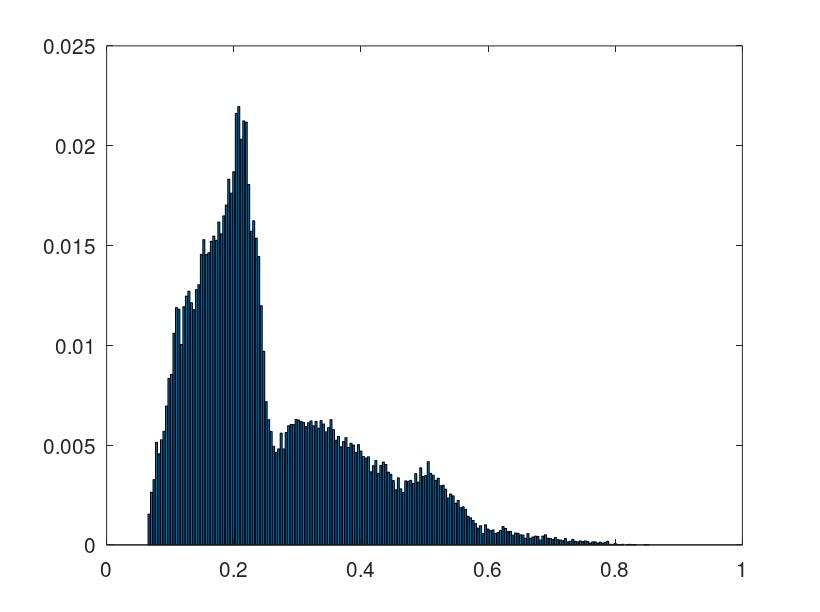
\includegraphics[width=80mm]{./img/flatten_ex.jpg}
    \caption{明るさにばらつきのある画像のヒストグラム}
    \label{hist_2}
\end{figure}

このようなヒストグラムに対して、ヒストグラムの山を広げるような処理をするのがヒストグラム平坦化である。

ヒストグラムの山を広げるという処理は線形濃度変換のようなシンプルなマッピング関数では実装が難しい。
そのため、ヒストグラム個別にマッピング関数を生成する必要がある。

このマッピング関数$f(x)$を求めるのは、複雑ではない。ヒストグラムの勾配が大きいところほど大きな山ができていることを
考えれば、このヒストグラム関数$h(x)$を単に積分してしまえばよい。
すなわち式にして表すと適当な0以上の係数$s$を用いて、式(5)のようになる。
\begin{equation}
    f(x) = s \int h(x)dx
\end{equation}

ただしヒストグラム関数が離散値であるので
\begin{equation}
    f(x) = \sum_{i=i}^{x}h(i)
\end{equation}
とすることで、入力画像毎にマッピング関数を決めることができる。

実際にこの処理を画像に施すと図\ref{hist_3}のようなヒストグラムの変換を行うことができる
(図\ref{hist_3}では簡略化した数式で表している)。

\begin{figure}[htbp]
    \centering
    \begin{tabular}{ccccc}
    \begin{minipage}[l]{0.2\hsize}
        \centering
        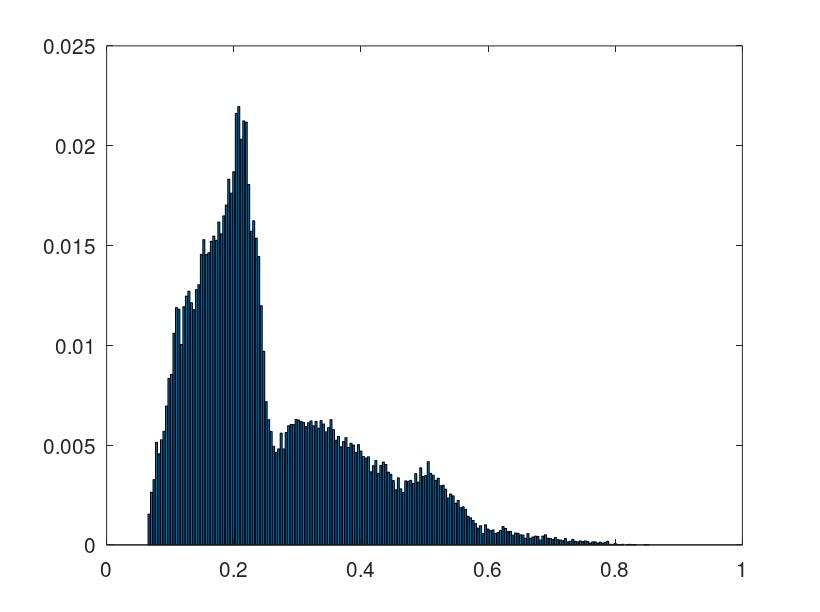
\includegraphics[width=40mm]{./img/flatten_ex.jpg}
    \end{minipage}&
    \begin{minipage}[c]{0.2\hsize}
        \centering
        \begin{math}
                \overset{f(x) = \sum_{i=i}^{x}h(i)}{\to}
        \end{math}
    \end{minipage}&
    \begin{minipage}[c]{0.21\hsize}
        \centering
        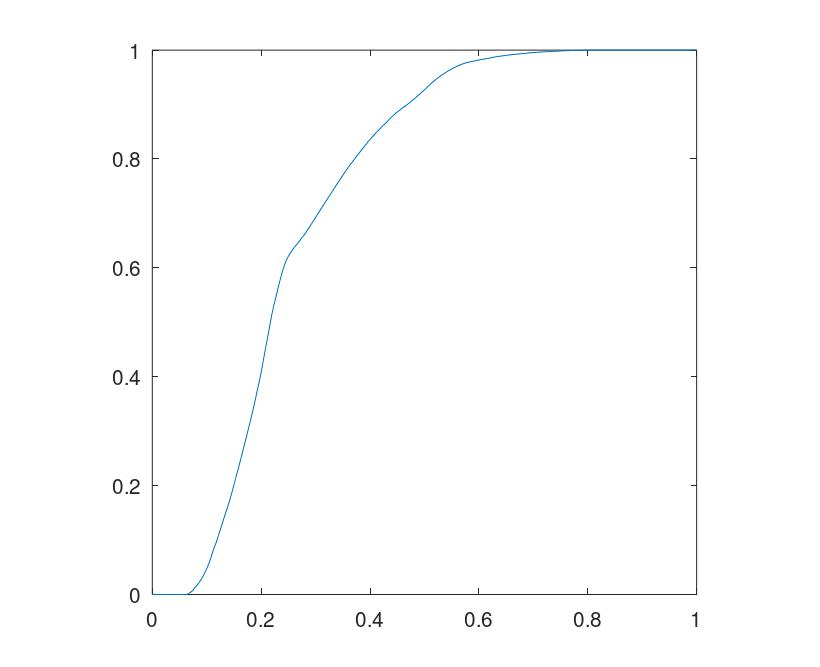
\includegraphics[width=30mm]{./img/flatten_func_ex.jpg}
    \end{minipage}&
    \begin{minipage}{0.12\hsize}
        \centering
        \begin{math}
                \overset{h'(x)=f(h(x))}{\to}
        \end{math}
    \end{minipage}&
    \begin{minipage}[c]{0.2\hsize}
        \centering
        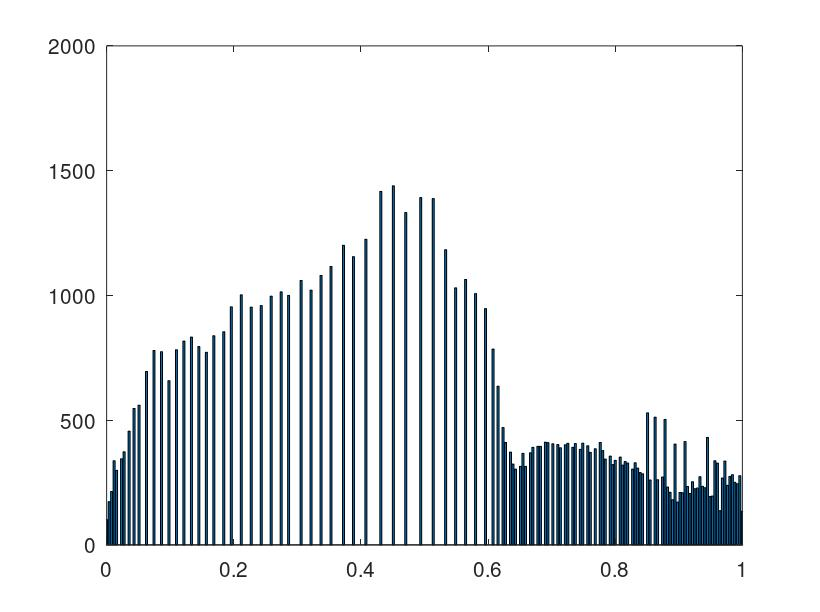
\includegraphics[width=40mm]{./img/flatten_ex2.jpg}
    \end{minipage}
    \end{tabular}
    \caption{ヒストグラム平坦化によるヒストグラムの変化例}
    \label{hist_3}
\end{figure}

これがヒストグラム平坦化の処理内容となる。

\section{演習-考察}
では実際に、画像に対してヒストグラムの線形濃度変換とヒストグラム平坦化の処理を行い、
その処理で当該画像がどのように変化したのかを考える。

\subsection{線形濃度変換}
まず、線形濃度変換から行う。

図\ref{Morita}のような画像を用意した。これは上田市駅近くにある町中華モリタである。
\begin{figure}[htbp]
    \centering
    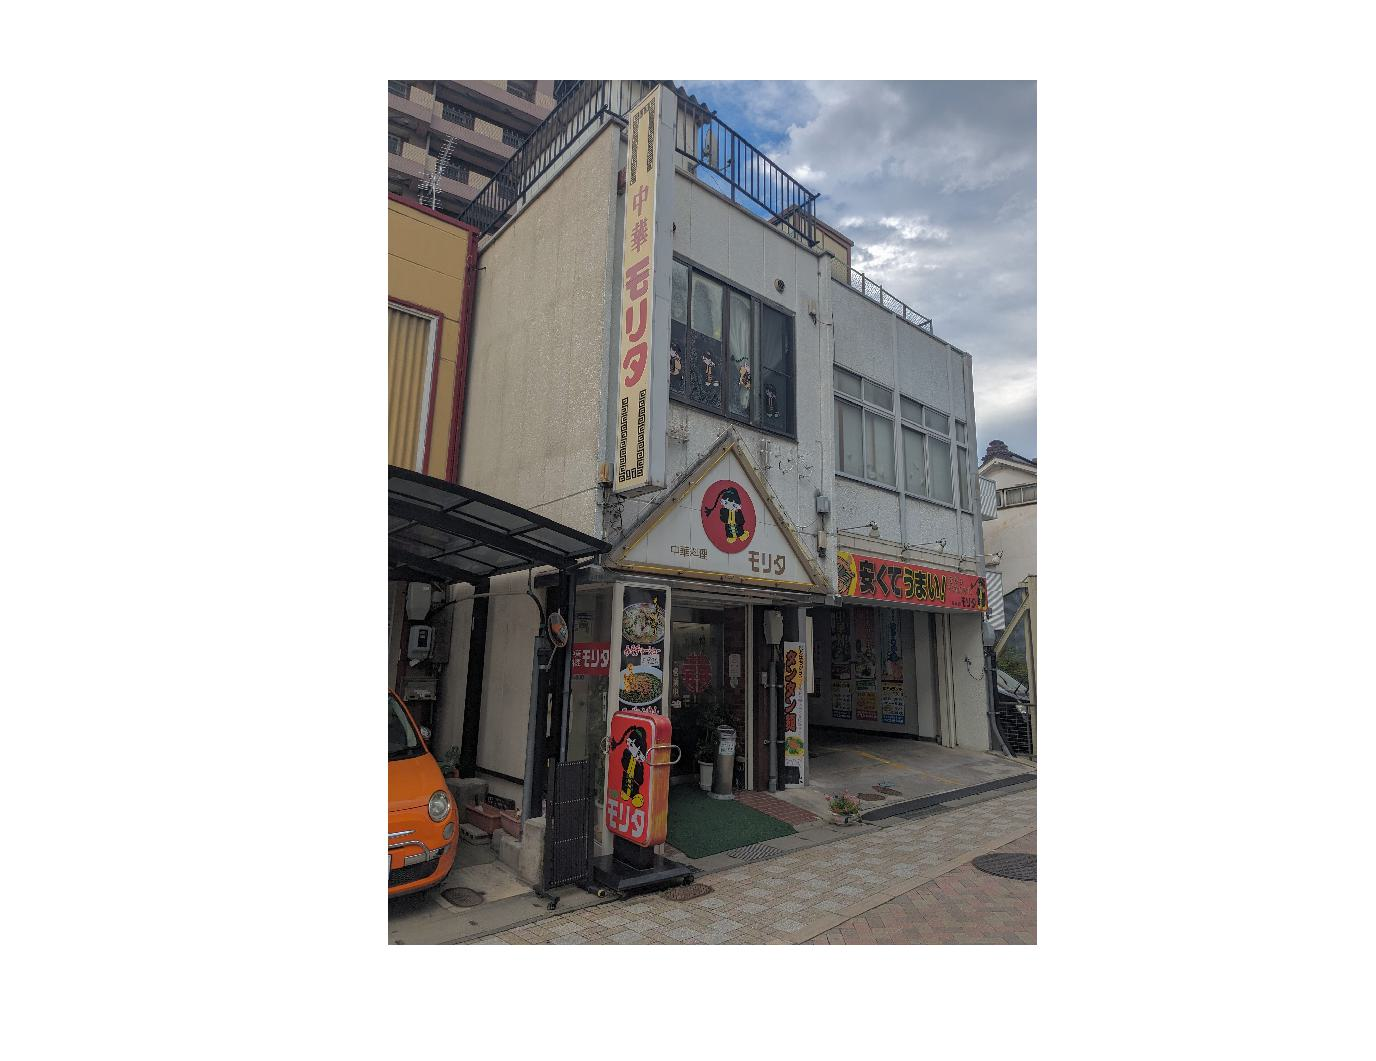
\includegraphics[width=120mm]{./img/linear_beforeimg.jpg}
    \caption{線形濃度変換を行う前の画像}
    \label{Morita}
\end{figure}

図\ref{Morita}の画像は雲の色や建物の色など、少しはっきりとしない部分が多く、コントラストが低くなっていることがわかる。

\newpage
実際にヒストグラムを出力してみると図\ref{bfhist}のように輝度値の範囲が狭くなっていることが分かる。
\begin{figure}[htbp]
    \centering
    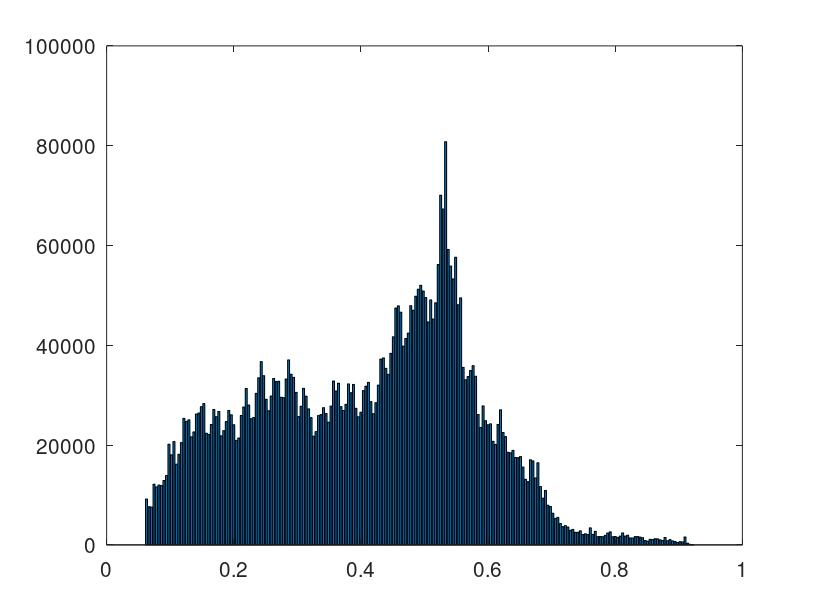
\includegraphics[width=80mm]{./img/linear_beforefunc.jpg}
    \caption{線形濃度変換を行う前の画像(図\ref{Morita})のヒストグラム}
    \label{bfhist}
\end{figure}

これを線形濃度変換で輝度値の範囲を広くしていく。

処理前の輝度値の範囲はおよそ0.06~0.91である。この範囲を0~1に広げたいので$x_1=0.06,x_2=0.91,y_1=0,y_2=1$
として式(4)を使って$y=ax+b$の定数部分を求めれば$a\simeq 1.17,b\simeq -0.07$となるので
$y=1.17x-0.07$の関数を用いて変換を行えばよい。

実際に変換を行うとヒストグラムは図\ref{afhist}のように出力された。
\begin{figure}[htbp]
    \centering
    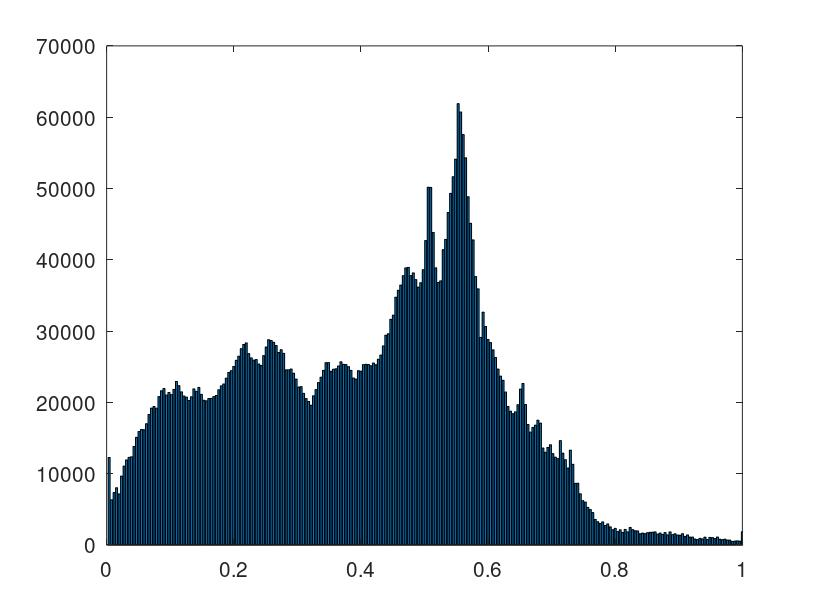
\includegraphics[width=80mm]{./img/linear_afterfunc.jpg}
    \caption{線形濃度変換を行ったあとの画像のヒストグラム}
    \label{afhist}
\end{figure}

図\ref{afhist}を見れば分かるようにヒストグラムが輝度値いっぱいに展開されていることが分かる。

\newpage
この線形濃度変換を行った画像が図\ref{afMorita}になる。
\begin{figure}[htbp]
    \centering
    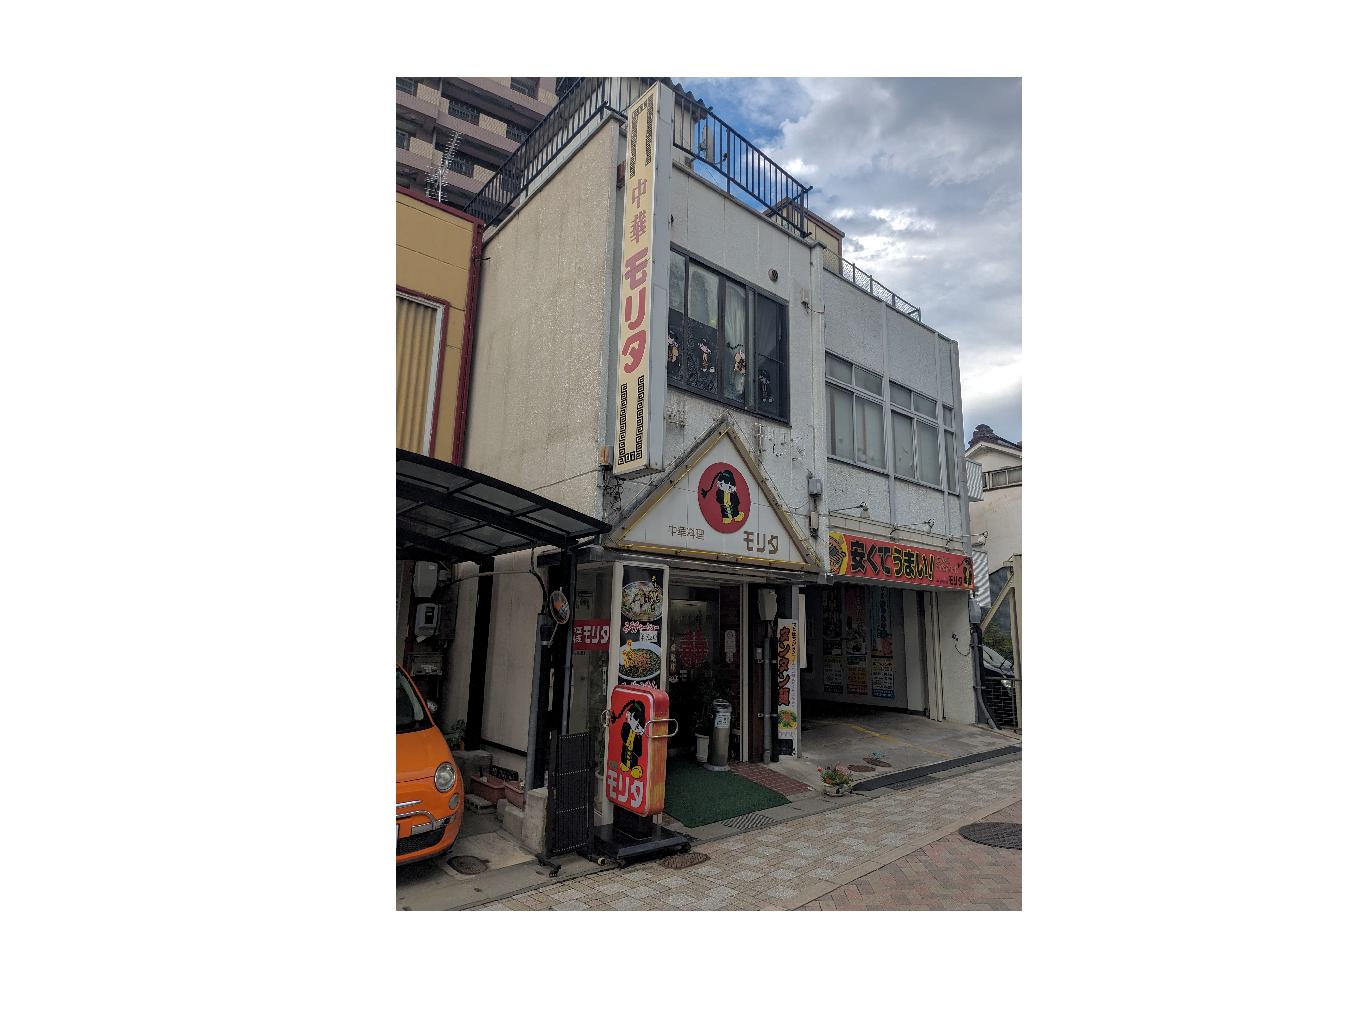
\includegraphics[width=120mm]{./img/linear_afterimg.jpg}
    \caption{線形濃度変換を行った後の画像}
    \label{afMorita}
\end{figure}

処理前と処理後で画像を比較すると図\ref{conimg}のようになる。
\begin{figure}[htbp]
    \centering
    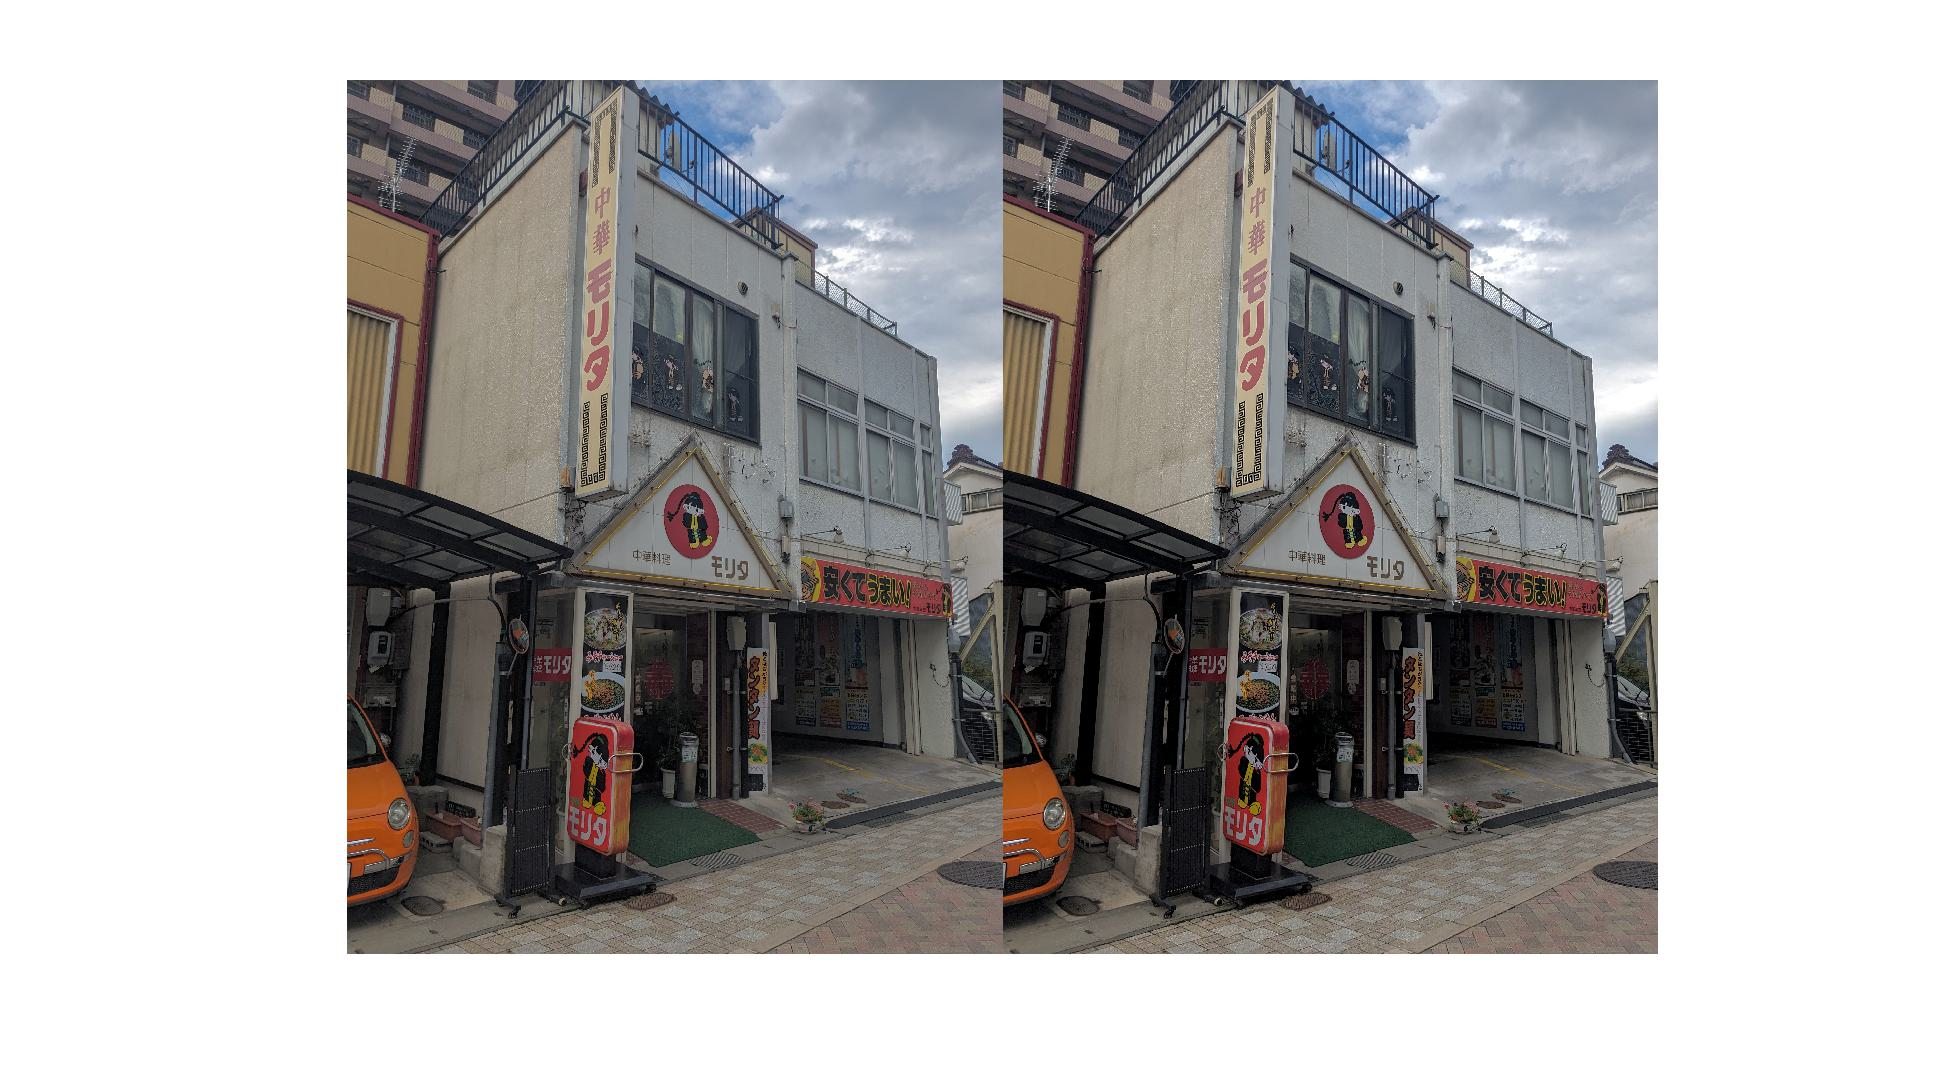
\includegraphics[width=120mm]{./img/linear_imgcon.jpg}
    \caption{処理前後の画像比較(左が処理前、右が処理後)}
    \label{conimg}
\end{figure}

こう比較すると元画像の輝度値がそこまで酷く狭いわけではなかったためわかりずらいが、
確かにコントラストに補正が入りはっきりとした画像になっていることが分かる。

\subsection{ヒストグラム平坦化}
続いてヒストグラム平坦化を行う画像は図\ref{MtIbuki}である。これは私が岐阜県の伊吹山へ行ったときに撮った写真である。
\begin{figure}[htbp]
    \centering
    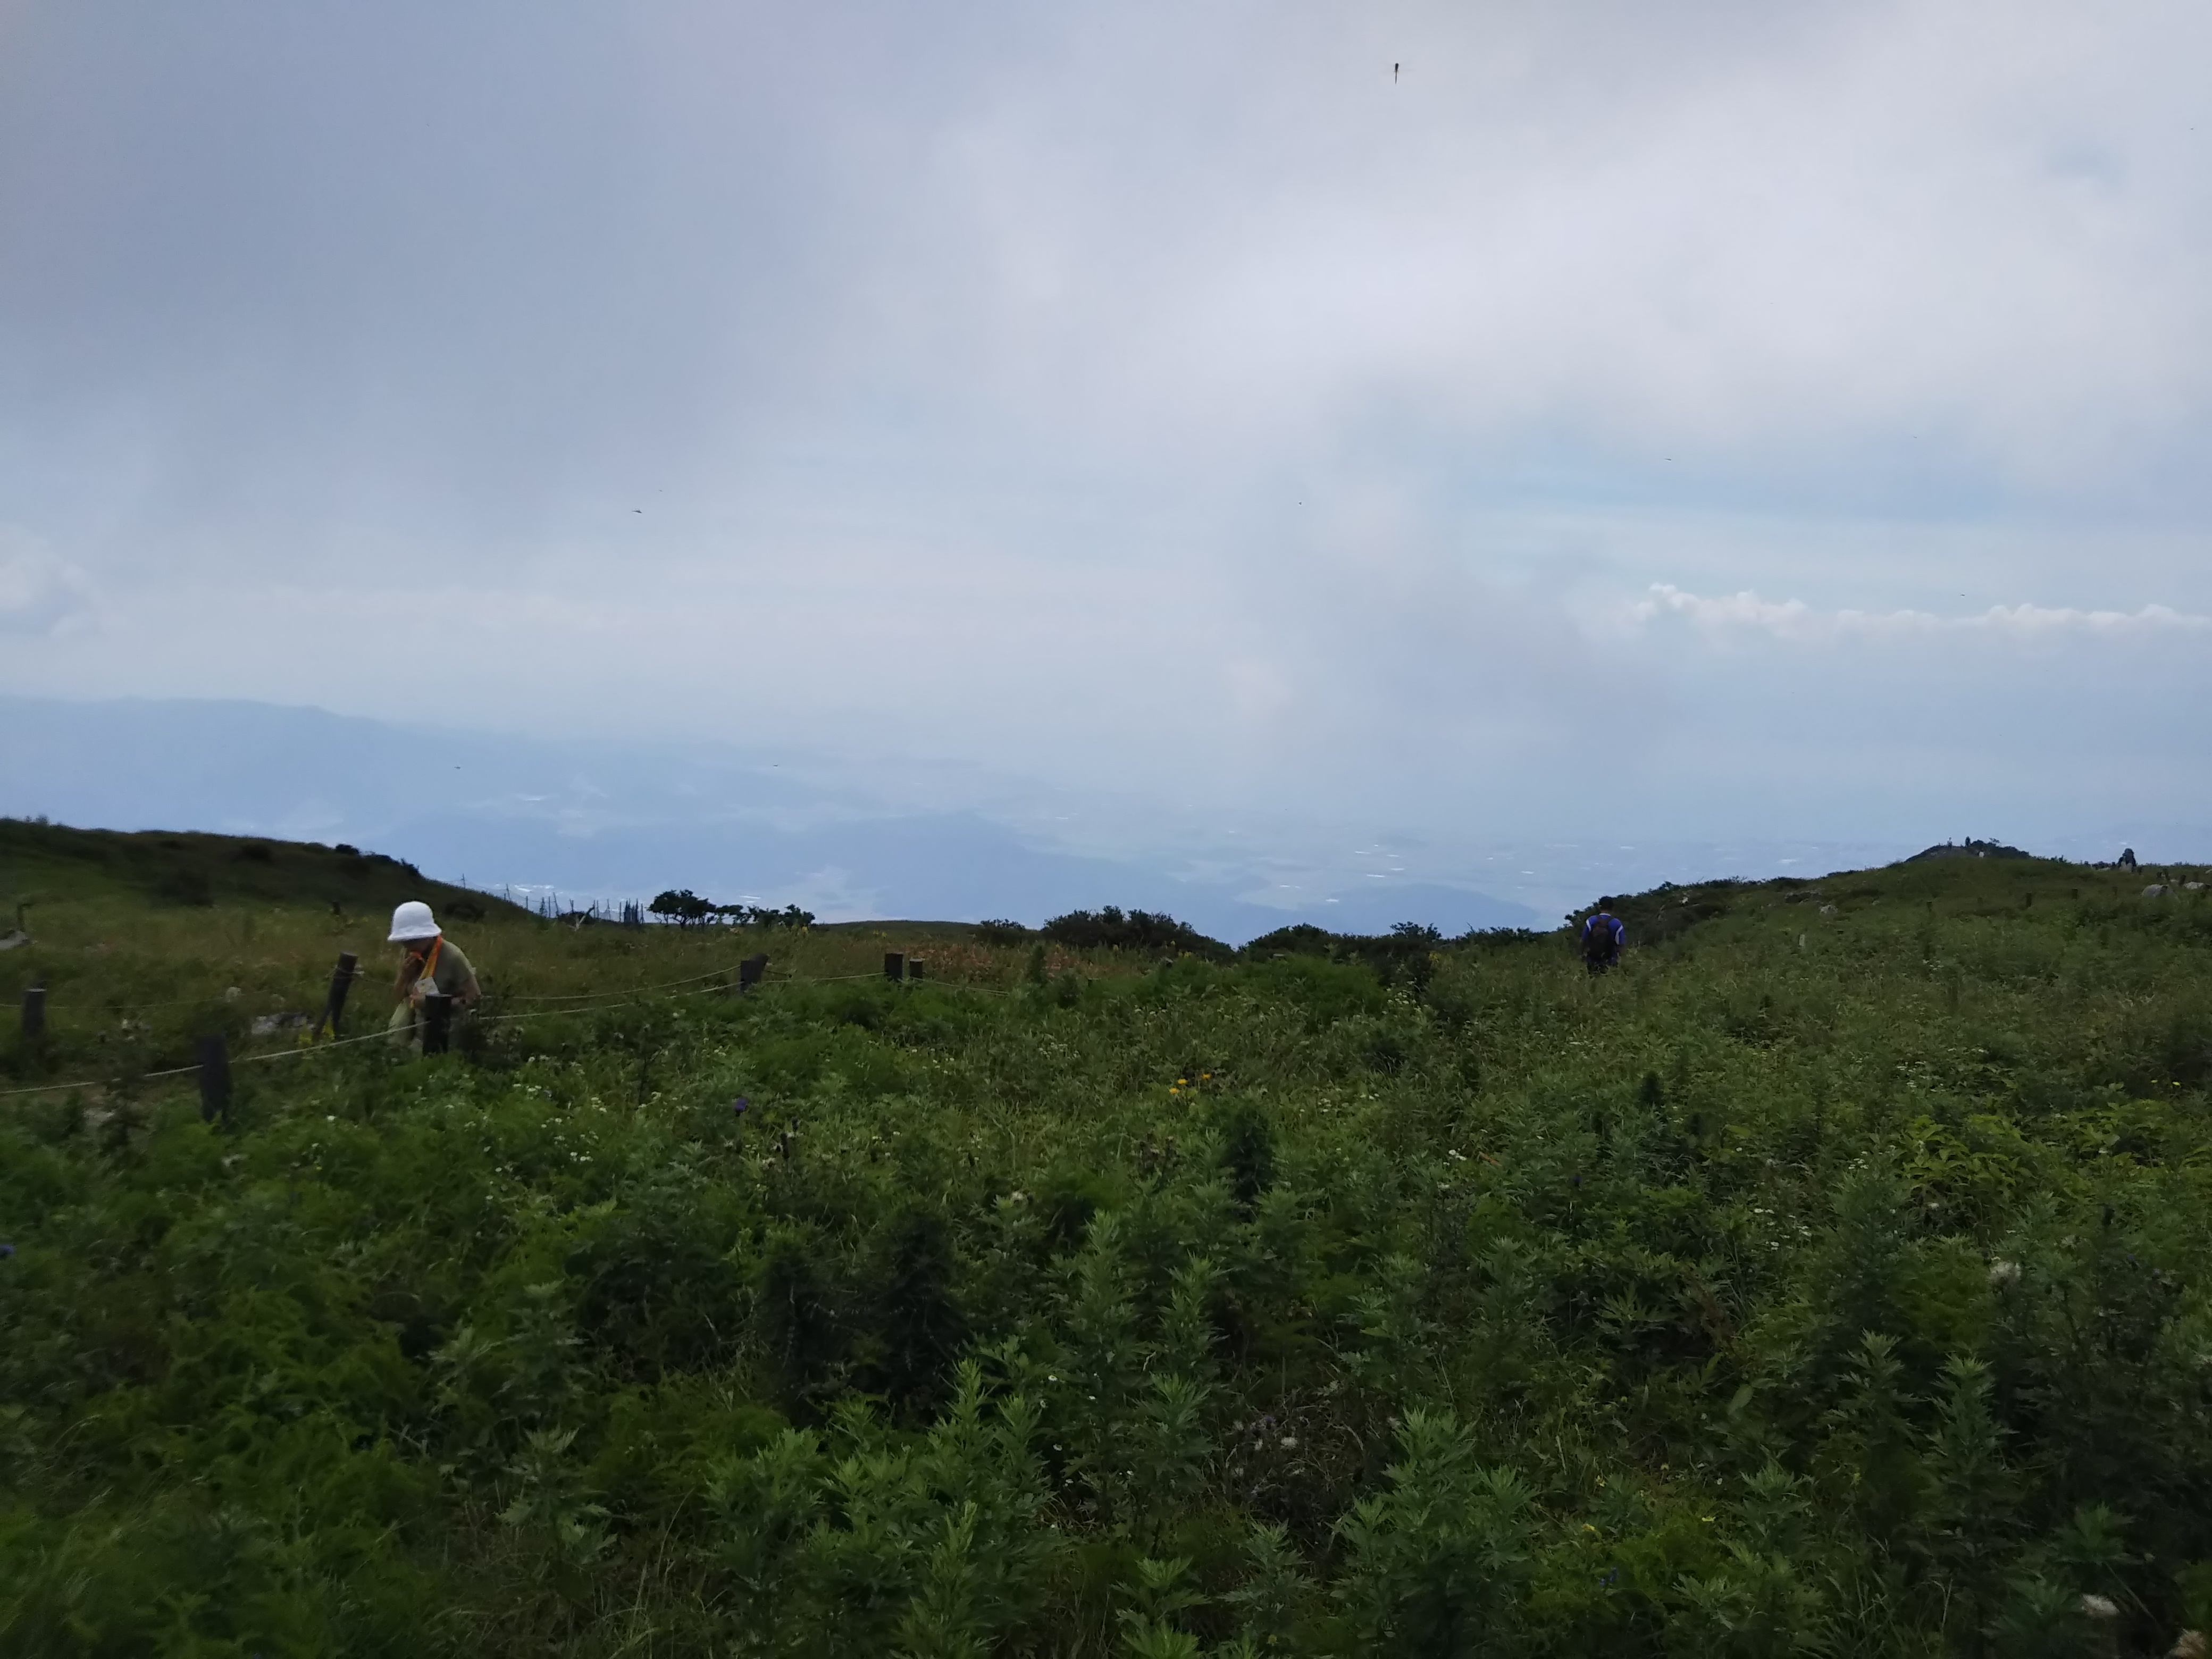
\includegraphics[width=60mm]{C:/Users/user/Documents/ImageProc/task/img/MtIbuki.jpg}
    \caption{ヒストグラム平坦化を行う前の画像}
    \label{MtIbuki}
\end{figure}

この画像は一見明るさのばらつきが酷くないが、ヒストグラムを見ると図\ref{bfhist_2}のように
大きな輝度値のピークを暗いところと明るいところに2つ確認できる。
\begin{figure}[htbp]
    \centering
    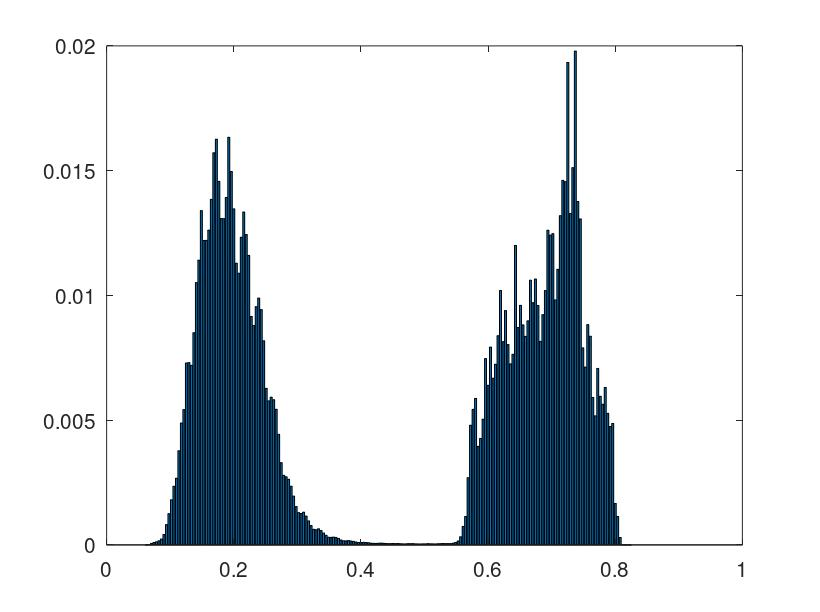
\includegraphics[width=80mm]{./img/flatten_beforefunc.jpg}
    \caption{処理前の図\ref{MtIbuki}のヒストグラム}
    \label{bfhist_2}
\end{figure}

これをヒストグラム平坦化にかけると図\ref{afhist_2}のヒストグラムと図\ref{afMtIbuki}の出力画像が得られる。
\begin{figure}[htbp]
    \centering
    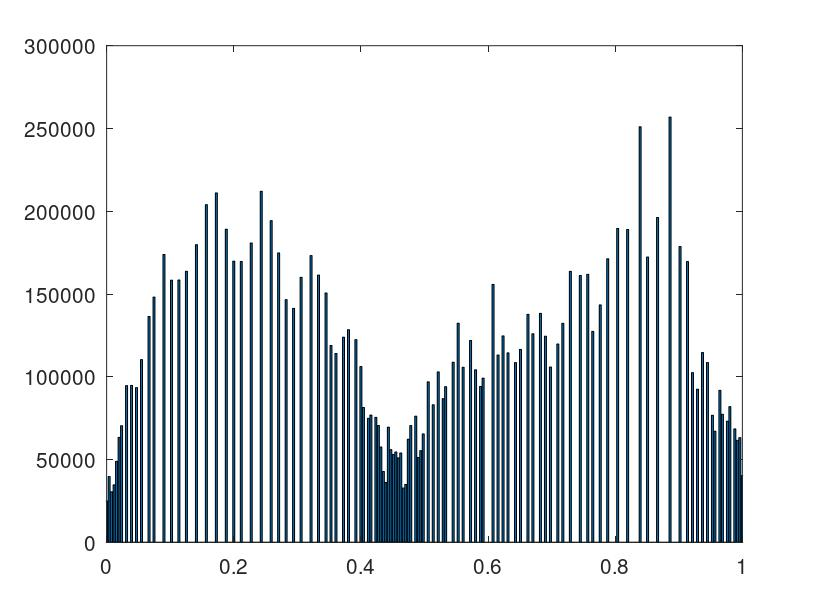
\includegraphics[width=80mm]{./img/flatten_afterfunc.jpg}
    \caption{処理後の図\ref{afMtIbuki}のヒストグラム}
    \label{afhist_2}
\end{figure}
\begin{figure}[htbp]
    \centering
    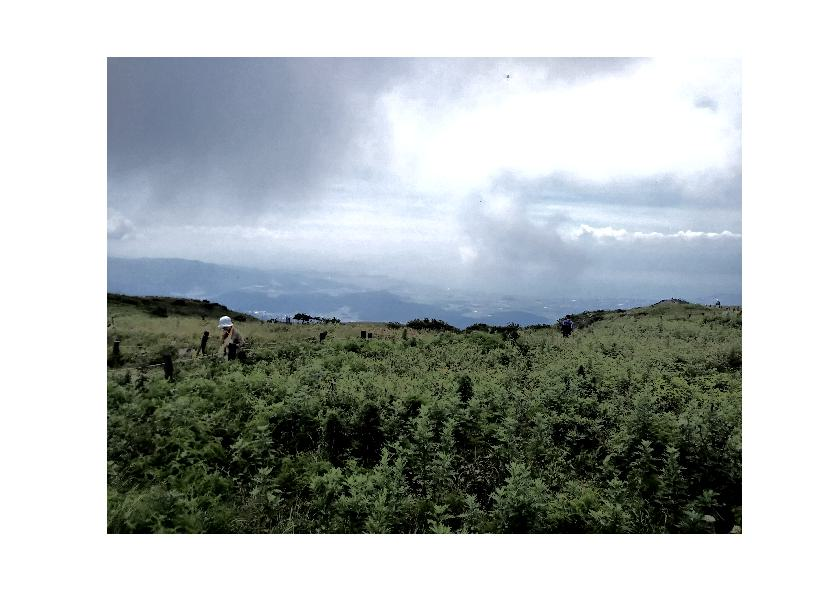
\includegraphics[width=80mm]{./img/flatten_afterimg.jpg}
    \caption{ヒストグラム平坦化を行った後の画像}
    \label{afMtIbuki}
\end{figure}

図\ref{bfhist_2}と図\ref{afhist_2}を比較するとわかるがヒストグラムにあったピークがかなり広がり、
勾配が緩やかになったことが分かる。また、図\ref{bfhist_2}では狭かった輝度値の範囲も図\ref{bfhist_2}
ではヒストグラム平坦化を施したことで大きく広がっていることが分かる。

また結果として出力された図\ref{afMtIbuki}は全体的に明るくなり、
逆光画像の影部分のようになっていた手前の草むらや雲もくっきりと見えるようになった。
画像自体が明るくなっているのは輝度値の範囲が広がったことにあると思うが、
輪郭のぼんやりしていた空が明るくなっているのはヒストグラム平坦化によるものだと考えられる。

\section{実験に用いたコード}
最後にこの実験にて用いたコードを示す。

\lstinputlisting[caption={線形濃度変換}]{c:/Users/user/Documents/ImageProc/task/lesson2_1.m}
\lstinputlisting[caption={ヒストグラム平坦化}]{c:/Users/user/Documents/ImageProc/task/lesson2_3_1.m}


\end{document}